\documentclass[10pt,a4paper]{article}

\usepackage{graphicx} % for inputing graphics
\usepackage{epstopdf} % Helper Package to graphix package
\usepackage{fancyvrb} % for \VerbatimInput (the nice inline code refrences)
\usepackage{amssymb} % American Math Society package, creates theorems and more math things 
\usepackage{caption} %creates captions for figures and other floating objects in paper 
\usepackage[fleqn]{amsmath} %flegn- moves equations to the left amsmath-helps with equation building other math things
\usepackage{tipa} % imports greek characters and other random letters heres a cool cheat sheet! https://ptmartins.info/tex/tipacheatsheet.pdf
\usepackage{tipx} % additional font comands for the tipa package. not 100%
\usepackage{breakcites} % an asthetics feather that makes a line break after citations 
\usepackage{makeidx}
\usepackage[hyperpageref]{backref}
\usepackage{graphics}
\usepackage{enumitem}
\usepackage{float}
\usepackage[T1]{fontenc}
\usepackage[utf8]{inputenc}
\usepackage{authblk}
\usepackage{booktabs}
\usepackage{a4wide}

\usepackage{color}
\definecolor{MyDarkGreen}{rgb}{0.0,0.4,0.0}
\definecolor{MyDarkRed}{rgb}{0.4,0.0,0.0} 
\definecolor{MyBlue}{rgb}{0.0, 0.0, 0.5} 
\definecolor{MyOrange1}{rgb}{1.0, 0.9, 0.0} 

\usepackage[colorlinks=true, urlcolor= MyBlue, linkcolor= MyBlue, citecolor=MyDarkGreen ]{hyperref}

\setcounter{secnumdepth}{3}
\setcounter{tocdepth}{3}
\makeindex

\DeclareCaptionLabelSeparator{space}

\DeclareGraphicsRule{.tif}{png}{.png}{`convert #1 `dirname #1`/`basename #1 .tif`.png}
\textwidth = 6.5 in
\textheight = 8.2 in
\oddsidemargin = 0.0 in
\evensidemargin = 0.0 in
\topmargin = 0.0 in
\headheight = 0.0 in
\headsep = 0.7 in
\parskip = 0.2in
\parindent = 0.0in

% defining thorems corollarys and definitions 
\newtheorem{theorem}{Theorem}
\newtheorem{corollary}[theorem]{Corollary}
\newtheorem{definition}{Definition}

\setlength{\parindent}{1cm}
\newcommand{\abstractinenglishname}{Abstract}
\newenvironment{abstractinenglish}{
        \def\abstractname{\abstractinenglishname}
	\begin{abstract}
}{
        \end{abstract}
}

\title{Applications of Natural Language Processing to Compare Shakespearean Sonnets to Modern Musical Artists}
\author[*]{Mariana Gonzalez Castro}
\author[*]{Carina Kalaydjian}
\author[*]{Dominique McDonald}
\author[*]{Angel Sierra}
\author[*]{DuoDuo Ying}
\affil[*]{Department of Statistics, UCLA}

\date{June 8th, 2022}
%%%%%%%%%%%%%%%%%
%	HELPFUL BIBLIOGRAPHY KEY
% Here im going to list all the bibliography entries refnrece names and a short description of what the refrence is refrencing. 
% This way, all the refrences are here and no need to look back and forth to the bib file to cite stuff
%
% example: \cite{monkey} will cite "what is tech analysis a begginers guide", from monkeylearn.com
%
% refrence name - description
% monkey - what is tech analysis a begginers guide, monkeylearn.com
% web1 - Natural Language Processing with R,  Udacity.com  
% web2 - text mining and sentiment analysis: analysis with R, red-gate.com
% briney2015data - the briney book from class? i added it but not sure if we will need it 
% syuzhet - syuzhet package documentation in R 
% sonnetsData - refrences all of shakespears sonnets from the gutenberg project
% musicData - Refrences kaggle dataset with the music artists and their lyrics
% tm - Tm: text mining package documentation in R
% shakeFacts - fun facts about william shakespear 
% scienceDirect - Chapter 4: Text Mining and Network Analysis of Digital Libraries in R
% k-means - K-means Clustering: Algorithm, Applications, Evaluation Methods, and Drawbacks, from towardsdatascince.com
% NLP-for-music - Natural language processing for music knowledge discovery, article 
% NLP-for-lyrics - Natural language processing of lyrics, article
% knowledge-graphs - An Introduction to Knowledge Graphs, from standord AI labs 
% nrc-sentiment - NRC Word-Emotion Association Lexicon
% music-world, NRC Word-Emotion Association Lexicon
% bio-article1 - authors Martín Nicolás Fasanelli, Pablo S. Milla Carmona, Ignacio María Soto, Diego Tomás Tuero
% bio-article2 - authors Katie Ovens, Farhad Maleki, B. Frank Eames and Ian McQuillan
%%%%%%%%%%%%%%%%%%

%Testing space 
\usepackage{float}

\usepackage{listings}
\lstset{
   breaklines=true,
   basicstyle=\ttfamily}

\begin{document}

\maketitle
\vspace{6pt}

\begin{abstractinenglish}
\emph{We seek to detect artists that are truly outstanding and stand the trial of time. In this paper, we introduced a metric to predict 45 artists’ success based on the similarity between a subset of their discography and Shakespeare’s 154 sonnets. We used Natural Language Processing, specially Keyword Extraction and Sentiment Analysis, to measure such similarities. For Keyword Extraction, we measured the number of similar top 10 keywords used between artists and Shakespeare and the Euclidean distance of the frequencies. For Sentiment Analysis, we performed a cluster analysis and measured the Euclidean distance for 8 emotions within the text of artists and Shakespeare. We combined the result for the two methodologies and their rankings to obtain an overall ranking. Out of 45 top artists, Nickelback, Amy Winehouse, and Cake are the most similar artists to Shakespeare using the combined ranking. We conclude that by leveraging Natural Language Processing algorithms, we can predict future success based on the proven success of the past. }
\end{abstractinenglish}

\section{Introduction}
% Example of how to refrence name of a code file in apendix 
% Examine and run \texttt{\char`_code\char`_A.R}
%
% Example of how to make latex print texts that looks like terminal commands 
% \begin{verbatim}
% install ccrypt
% \end{verbatim}

%example of how to insert a picture
%\begin{center}
%\includegraphics[width=14cm]{_assets/*some name*.png}
%\end{center}

%%%%%%%% Remove tester before submitting 
here we cite \cite{web1} our glorius leader \cite{web2} yeah yeah cool cool \cite{briney2015data} and this too \cite{monkey} this as well \cite{sonnetsData} woohooo!!! \cite{musicData} and \cite{syuzhet} and \cite{tm} and \cite{shakeFacts} sdljdj \cite{k-means} , \cite{NLP-for-music} and  \cite{NLP-for-lyrics}, \cite{knowledge-graphs}, \cite{nrc-sentiment}anan \cite{music-world}, \cite{bio-article1}, \cite{bio-article2}
%%%%%%%%%%%%%%%%%%

The music industry has been growing in popularity over the last few decades. In 2021, worldwide recorded music revenues totaled \$25.9 billion, up 18.5 percent from 2020. \cite{music-world}There are more and more artists representing different genres, styles, and even subgenres within genres. As a prominent music label, we wonder how to detect artists that are outstanding and stand the trial of time? Who are the artists that are not only relevant now but tens and hundreds of years from now?

\noindent In this paper, we propose a method for measuring artists’ timelessness using their similarities with Shakespeare. William Shakespeare is a world-renowned poet from 16th-century England. He has recognition for being one of the most revolutionary Literary Artists to this date. Not only has Shakespeare close to one-tenth of the most quoted lines ever written or spoken in English, second-most quoted after the writers of the bible, but his ability to deeply express emotions also has influenced for hundreds of years.\cite{shakeFacts} We assume that, given William Shakespeare’s success, if modern artists’ work is similar to that of William Shakespeare’s in terms of word choice and sentiment, then they are likely to be successful as well.

\noindent For our data, we use Shakespeare's 154 sonnets from the Gutenberg Project. \cite{sonnetsData} We obtained a subset of 45 top modern artists’ discography through a Kaggle competition. We will use Natural Language Processing, specifically Keyword Extraction and Sentiment Analysis, to measure similarities between the work of 45 artists and 154 sonnets of Shakespeare. The rest of the paper is structured as follows: Section 2 introduces the methodology, both the front-end analysis and back-end data management. Section 3 provides results and plots from our analysis. Section 4 concludes. Our code and Appendix can be found in Section 5. 

\section{Methods}
There is a growing demand for the application of Natural Language Processing to drive music knowledge discovery \cite{NLP-for-lyrics}. Within song lyrics there is a wealth of information that can be used to gain insights about the song and its listeners. The workflow used to conduct NLP is outlined in Oramas et. Al \cite{NLP-for-music} as the following steps 1. Corpus creation (collection of separated documents), 2. Text mining (accessing desired info and eliminating the excess), 3. Information extraction (word frequency, collocation, word position, etc.), 4. Knowledge graph generation (a directed labeled graph in which we have associated domain specific meanings with nodes and edges \cite{knowledge-graphs}), 5. Sentiment Analysis (Identify feelings and emotions present in a text \cite{monkey}).
 
\noindent This NLP pipeline can be applied to music to provide recommendations on what songs a listener might like based on what they already listen to. \cite{NLP-for-lyrics} This information is gathered by performing what’s called a similarity search. Mahedero et al \cite{NLP-for-lyrics} conducts a similarity search for their project by first calculating a similarity measure. The similarity measure used is known as the Standard Cosine Distance (SCD). The calculations of the SCD are beyond the scope of this paper, but something to note is that the SCD relies on the Inverse Document Frequency as a way to measure the prevalence of words in a document and compare that to other documents. 

\noindent As previously stated, we relied on Natural Language Processing methods to calculate the similarity between Shakespeare and current artists with the hope of identifying a single artist whose work has similar themes as Shakespeare’s. Our pipeline was structured similarly to that proposed in \cite{NLP-for-music} with the main difference being that we do not rely on knowledge graph generation to store any information or display findings. The methods that were most useful for this research were keyword extraction and sentiment analysis. Both methods of analysis provided us with crucial insights, so the details of each seem pertinent to share. 

\subsection{Keyword Extraction}
Keyword extraction is largely aimed at identifying the most relevant words in different texts and utilizing those words to understand common theme or popular topics.\cite{monkey} We used the tm library in R to perform keyword extraction\cite{tm} on the sonnets. This process involves first prepping the text by removing unwanted punctuation or numbers, eliminating stop words, changing everything to lower case. These transformations are necessary because when working with strings, you not only have to be precise, but you also must be exact. The cleaning process sometimes includes stemming the words, but we opted not to do that. Once the text is clean the idea is to create a table containing each word used in the text and the frequency with which it is used. To identify the top ten key words we sorted the words in the matrix by their frequency. 

%%%%%%%%%%% keywords shakespears wordcloud 
\begin{center}
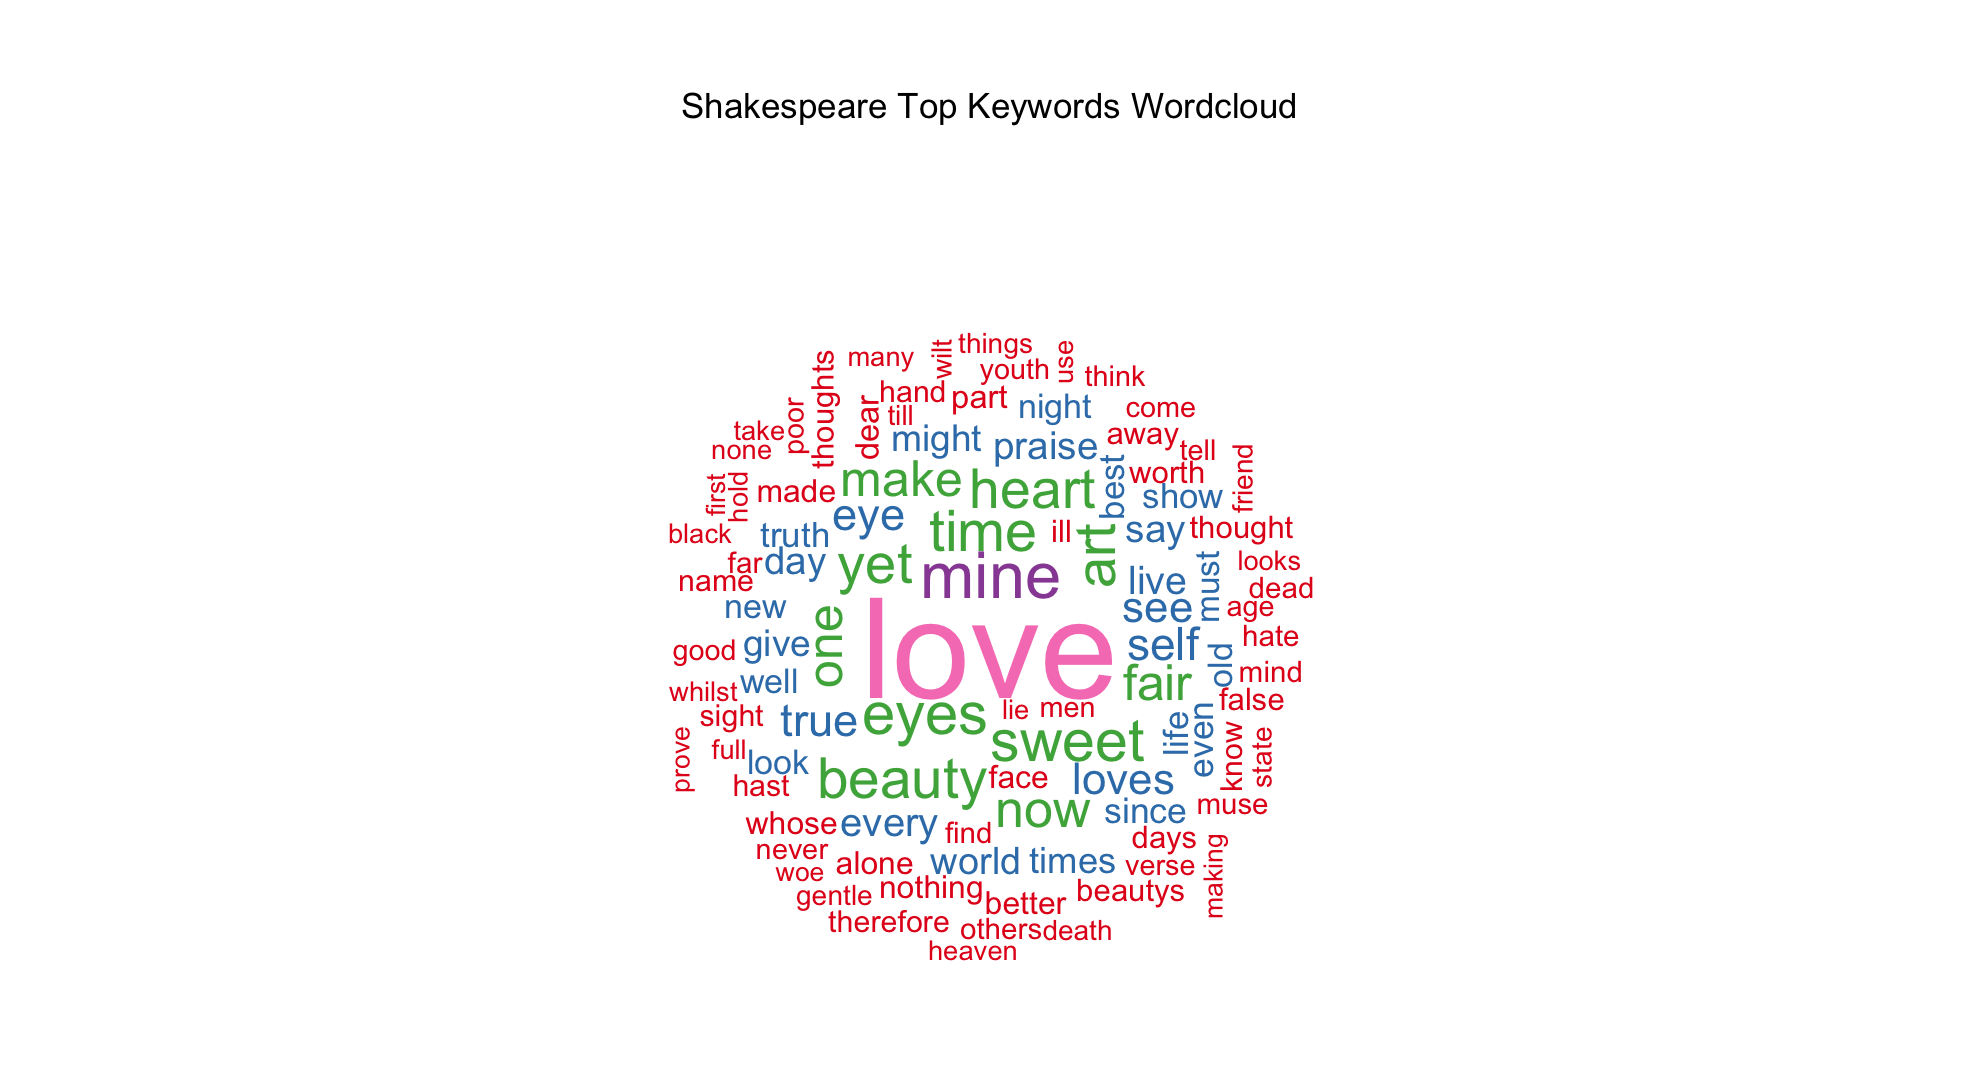
\includegraphics[width=14cm]{_assets/Shakespeare_Keywords_WordCloud.png}
\end{center}

\noindent Once Shakespeare’s keywords were identified, the next step was to identify the keywords for each of the 45 music artists. This process mirrored that of extracting keywords from the sonnets except we utilized an algorithm to automate the process for each artist. Once keywords were identified we converted the word frequencies for Shakespeare and all other artists into proportions, in order to standardize for comparison. To find the artists who were most like Shakespeare based on keywords, we checked for artist who had the highest number of matching keywords. Finally, then we ranked those by who used keywords in similar proportions to Shakespeare by calculating the Euclidian distance between the proportions of each of the matching keywords. This is similar to what Mahedero et. Al \cite{NLP-for-lyrics} does for their similarity search except we rely on word proportions and Euclidean distance, while their research utilizes Inverse Document Frequency and the Standard Cosine Distances. 

\subsection{Sentiment Analysis}
A similar sort of ranking was achieved from Sentiment Analysis, but the process has notable differences. The library syuzhet was used for the analysis. There is a wide variety of paths one could explore when performing sentiment analysis. Two that seemed viable for the purpose of this research were calculating an overall sentiment score and identifying the different emotions present in each text. \cite{syuzhet} The latter option proved to be more fruitful, as the analysis is more detailed. This process of classification based on emotion is known as NRC sentiment analysis. NRC Sentiment Analysis uses the National Research Council (NRC) Word-Emotion Association Lexicon to classify words in a text into eight categories of emotions. \cite{nrc-sentiment} It is important to note that a word may be associated with more than one emotion. The eight emotions are anger, anticipation, disgust, fear, joy, sadness, surprise, trust (include simple equation). \cite{nrc-sentiment} The objective of NRC Sentiment Analysis is to calculate the frequency with which each emotion is conveyed. This is calculated by identifying the emotions associated with the unique words in a text and summing up all the instances of each emotion\cite{syuzhet}. 

\noindent Once the NRC sentiments were calculated for both Shakespeare and the music artists, the frequencies were converted to proportions for accurate comparison. Using the proportions of each emotion, Euclidean distance was calculated for between each music artist and Shakespeare. The artists with the shortest distances from Shakespeare were considered the most similar to him, and therefore ranked higher in regard to comparison of the emotions conveyed in their works. 

\noindent After comparing results from each analysis method, a final ranking was calculated. This overall ranking was calculated by summing up the rankings from both analysis methods. Because similarity to Shakespeare was assessed using Euclidean distance, lower rankings signify higher similarity to Shakespeare. This meant that the artists with the lowest overall ranking mirrored Shakespeare’s work emotionally more than other artists.

\subsection{K-Means Clustering}
The NRC sentiments were utilized even further as predictors in K-Means Cluster Analysis. The objective of cluster analysis within the scope of this research is to utilize an unsupervised learning model \cite{k-means} to assess commonalities between the work of each music artist and Shakespeare. K-Means clustering is an iterative method that categorizes each data point into one of k predefined groups, or clusters. The process is driven by two objectives. The first being maximizing the distance between clusters, so that they are distinct. The second is minimizing the data points within a cluster, so the clusters themselves are homogenous. \cite{k-means} By employing K-means Clustering we were able to identify a group of artists that whose work most closely matches Shakespeare’s. 

\subsection{Data Management}
Before discussing the results of our various methods, it is important to address what made such an undertaking possible: data management.  The size of this project necessitated multiple team members using multiple platforms. The data was stored in a relational database and then hosted on  Amazon Web Services(AWS) service called Relational Database Services(RDS). Using RDS preserves the database from alterations, each memeber each member provided the read only user credentials to their database to enable the team to access data without making changes to the database itself. Once we had the data it the next steps were to process and analyze it. 

\noindent Again, with so many contributors working to advance the project it was necessary to have an avenue for efficient and organized sharing of code. For this aspect of the project, GitHub was utilized and it allowed team members to work on the same files from different locations and share them as frequently as necessary. Along with our code we are also able to store and share important information that aided us in our research. The different information sharing structures employed allowed for efficient progression and ultimately valuable results. 

%%%%%%%%%%%%%%%%%%%%%%%%%
\section{Results}
Natural Learning Process requires the creation of a corpus to perform keyword extraction and sentiment analysis on the sonnets of Shakespeare. Separate corpora of 45 sampled musical artists were made to perform more keyword extraction and sentiment analysis for comparison to Shakespeare. Shakespeare’s sonnets were collapsed such that a single corpus contained all 154 sonnets, each line representing a single line from a single sonnet. Each of the 45 artists had associated with a single corpus that contained multiple songs of their total discography, with each line representing a single line from a single song for the respective artist. With such corpora made, analysis of the text may begin.

\newpage
%%%%%%%%%% all rankings table
\begin{table}[ht]
\centering
\begin{tabular}{lrrr}
  \hline
Artist & Word Rank & Sentiment Rank & Overall Rank \\ 
  \hline
amy-winehouse &   6 &   1 &   7 \\ 
  nickelback &   2 &   8 &  10 \\ 
  cake &   9 &   3 &  12 \\ 
  adele &   1 &  21 &  22 \\ 
  joni-mitchell &  11 &  11 &  22 \\ 
  leonard-cohen &   8 &  15 &  23 \\ 
  paul-simon &  10 &  22 &  32 \\ 
  blink-182 &  18 &  14 &  32 \\ 
  bob-marley &  27 &   6 &  33 \\ 
  rihanna &  25 &  10 &  35 \\ 
   \hline
\end{tabular}
\caption{Ranked Top 10 Most Similar Music Artist to Shakespeare} 
\label{tab:overallranktable}
\end{table}



\noindent Keyword extraction and sentiment analysis of Shakespeare’s 154 sonnets against the discography of 45 sampled musical artists allow for an ordinal ranking of the artists in terms of similarity with Shakespeare. Amy Winehouse ranks most like Shakespeare considering a combined analysis. This can be interpreted as Amy Winehouse being most similar to Shakespeare in terms of keywords used by both persons and in terms of the eight measured emotions (anger, anticipation, disgust, fear, joy, sadness, surprise, trust) exhibited by their respective bodies of work. Shakespeare frequently writes about love, as seen in the keyword extraction of his sonnets. “Love” is also a keyword for Amy Winehouse. As for sentiment, Shakespeare and Amy Winehouse’s bodies of work display a similar amount of the eight mentioned emotions being measured, relative to the other 44 musical artists. Essentially, of the 45 musical artists being examined, Amy Winehouse writes about the same topic in the most similar manner to Shakespeare.

%%%%%%%%%%%%%% include keyword rankings table here
\begin{table}[ht]
\centering
\begin{tabular}{lrrlr}
  \hline
Artist & Word Count & Frequency & Keyword & Word Rank \\ 
  \hline
adele &   3 & 626.00 &  love time heart &   1 \\ 
  nickelback &   3 & 11349.00 &  love time yet &   2 \\ 
  bieber &   2 & 648.00 &  love time &   3 \\ 
  dolly-parton &   2 & 685.00 &  love time &   4 \\ 
  dj-khaled &   2 & 928.00 &  mine time &   5 \\ 
  amy-winehouse &   2 & 3700.00 &  love time &   6 \\ 
  bjork &   2 & 5341.00 &  love yet &   7 \\ 
  leonard-cohen &   2 & 5972.00 &  love time &   8 \\ 
  cake &   2 & 7690.00 &  love time &   9 \\ 
  paul-simon &   2 & 8464.00 &  love time &  10 \\ 
   \hline
\end{tabular}
\caption{Ranked Top 10 Most Similar Music Artist to Shakespeare Based on Keywords} 
\label{tab:wordranktable}
\end{table}



\noindent Keyword extraction alone allows for insight into which of the 45 sampled musical artists are most similar to Shakespeare’s sonnets in terms of theme. The artist Adele ranks most similar to Shakespeare when considering only keyword extraction. This can be interpreted such that both Shakespeare and Adele write about similar themes in their works. For example, Shakespeare and Adele have the keywords “love” and “heart,” and they both indeed write about facets of love. While Adele ranks highest among the 45 sampled musical artists, she ranks 21st in terms of sentiment. So while Shakespeare and Adele both may write about similar topics, the emotions expressed in their works differ enough to place Adele as 4th overall ranked in similarity to Shakespeare. This makes sense, as Adele tends to write about the frustrations and anxieties of love, while Shakespeare tends to write about the joys and excitement associated with love. 

%%%%%%%%%%%  sentiment analysis ranking table 
 \begin{table}[ht]
\centering
\begin{tabular}{lrr}
  \hline
Artist & Sent. Euclidean Distance & Sentiment Rank \\ 
  \hline
eminem & 0.00 &   1 \\ 
  nirvana & 0.00 &   2 \\ 
  cake & 0.00 &   3 \\ 
  amy-winehouse & 0.00 &   4 \\ 
  bob-dylan & 0.00 &   5 \\ 
  bob-marley & 0.00 &   6 \\ 
  johnny-cash & 0.00 &   7 \\ 
  nickelback & 0.00 &   8 \\ 
  britney-spears & 0.00 &   9 \\ 
  rihanna & 0.00 &  10 \\ 
   \hline
\end{tabular}
\caption{Ranked Top 10 Most Similar Music Artist to Shakespeare Based on Sentiments} 
\label{tab:wordranktable}
\end{table}

 

\noindent Sentiment analysis alone allows for insight into which of the 45 sampled musical artists are most similar to Shakespeare’s sonnets in terms of how the emotions anger, anticipation, disgust, fear, joy, sadness, surprise, and trust are expressed. Bob Dylan ranks as most similar to Shakespeare when considering only sentiment. In analyzing the sentiment Shakespeare expresses in his sonnets, all 154 poems were collapsed into a single corpus. This resulted in an analysis that concludes that Shakespeare’s most observed emotions are sadness, fear, and trust. While the poetry of Shakespeare is often not associated with such emotions, the manner of the analysis reveals that the work of Bob Dylan is associated with the emotions of fear, trust, and sadness, respectively. Bob Dylan tends to write songs of political engagement and the want for change, so his body of work reflecting such emotions seems to correlate appropriately. 

%%%%% kluster analysis table 
\begin{center}

\includegraphics[width=14cm]{_assets/ClusterAnalysis_Fit10.png}
\end{center}

\noindent Sentiment analysis of the 45 sampled artists were also implemented in k-means cluster analysis . Ten separate clusters were determined with Shakespeare being seen in the bottom right corner cluster, in blue. Notably, Bob Dylan and Amy Winehouse are in the same cluster as Shakespeare. This, naturally makes sense since both are highly ranked as being similar to Shakespeare in terms of sentiment analysis. 

\section{Conclusions}
In order to compare the Elizabethan works of Shakespeare to the modern musical artists of today, Keyword extraction and Sentiment analysis were used to compare Shakespeare’s original 154 sonnets to the bodies of work of 45 sampled artists. Keyword extraction, alone, revealed that Adele is most similar to Shakespeare with crossover words including “heart” and “love,” while sentiment analysis on its own revealed that Bob Dylan is most similar to Shakespeare. Combined keyword extraction and sentiment analysis show that Amy Winehouse is most similar to Shakespeare, since she ranked 4th most similar to Shakespeare in terms of keyword extraction and 5th most similar to Shakespeare in terms of sentiment. 

\noindent The 154 sonnets were all collapsed into a single corpus for analysis. If the sentiment analysis is done on the corpora of sonnets and not a single corpus, Shakespeare’s sentiments tend to be more positive, with joy and trust being the most common emotions. If the sentiment analysis is done on a single corpus of all the sonnets, Shakespeare’s sentiments tend to be more negative, with fear and sadness being the most common emotions. This inconsistency can be seen as a limitation of the study. The sentiment analysis done also did not include the positive and negative measures of analysis. Including these measures in future analysis could provide insights not otherwise seen. For future research, one solution would be to not collapse the sonnets and instead perform sentiment analysis on each individual sonnet and add up the 154 sentiment scores. A concern of this would be that if the sonnets were not collapsed into a single corpus, why collapse the songs of the 45 sampled artists. In experimenting with the methodologies, it was observed that collapsing the songs of the artists and not collapsing the sonnets resulted in sentiment analysis that is more easily interpretable. Future analysis would need to determine the exact effect collapsing all the work of a single artist has on the sentiment analysis of the corpus. 

\noindent Since the bodies of works of each artist were provided as a single corpus, there was no feasible way to separate the corpus into individual songs. This limitation prevented the possibility of performing sentiment analysis on individual songs. A continuation of this project would need to find an automated method to separate the songs from each other for a given artist. One possible method includes a strict k-means clustering - like algorithm that would separate clusters based on criterion that would include repetition of lyrics (repeated chorus in a song would be an indicator of a single cluster), and sentiment associated with a single song. A BERT (Bidirectional Encoder Representations from Transformers) model could also be applicable here. If a BERT model determines the next line of a song to be probabilistic, it can be reasoned that it would be in the same song. Implementation of such an algorithm would allow for an automated way to separate the songs of the corpus.

\noindent Different dimensions could have been considered for cluster analysis as well. For example, the reading level associated with Shakespeare’s sonnets could have been considered and compared to the reading levels of the bodies of work of the 45 artists and plots of k means cluster analysis could have been made. Other dimensions include line compositions such as the amount of type of word (adverb, adjective, noun), popularity of an artist compared to the popularity of sonnet, and use of punctuation. 

\noindent Notably, some of the songs in the bodies of work of the musical artists contained lyrics or songs in different languages. Theoretically, this would have little effect on the sentiment analysis, but the methodology applied does not support cross language analysis. Because of this, it would be necessary to translate the lyrics to English, for more proper sentiment analysis. This could have had an effect on the keyword extraction as well. There could have been more instances of keywords that were not counted since they were not in English. Another worry could be the fact that Shakespeare’s sonnets are written in early modern english. This makes it difficult to read and understand, and could have some influence on sentiment analysis. Solutions to this could include using new sonnets that translate the early modern Shakespearan sonnets to modern english. This could clarify the emotions of the sonnets, while not losing any meaning. 

\noindent Other methodologies could have been implemented as well to examine similarities among the corpora. Further emphasis could have been placed on n-grams to measure the collocation of keywords from the corpora. Identification of such collocated words would have allowed for a more accurate measure for keyword extraction, since collocated words are counted as a single word. The sonnets and bodies of works could have undergone tagging as well, where certain tags such as “nature”, or “love,” or “politics” could have been assigned to corpora that detail the theme of the work. A naive bayes classifier could then have been implemented to determine which sonnets belong to which tags and which sonnets correspond to artists that also possess similar tags. Finally, a BERT model could also be used in this scenario to provide a more complex methodology for sentiment analysis. BERT models often are used for next word predictions in text analysis, but a classification layer could be added on top of the transformer output to create a token for classification needs. 

\noindent The original idea of this project included the classification and analysis of synthetically made Shakespearean pseudo sonnets. A Markov Model was created and trained with the original 154 Shakespearean sonnets and then 5000 sonnets were created and stored on an off site location. Classification and analysis of these sonnets would include methodologies similar to those seen in this project, with sentiment analysis allowing for a thematic tagging of the pseudo sonnets. Classification trees could then be used to separate the pseudo sonnets. With appropriate tags associated with each pseudo sonnet, analysis would follow as frequency counts that could lead to regression analysis. Analysis could have gone as far as to see whether the tag frequencies of the generated sonnets were proportional to the tags of the original sonnets. Incorporation of these pseudo sonnets with the comparison of the 45 sampled artists would have also been possible. Similar analysis would be implemented on the individual songs of the artists that would then allow for a one to one association between pseudo sonnet and song. Based on analysis done with tagging and sentiment analysis, a model could theoretically provide similar pseudo sonnets and songs, given either an original sonnet or song.

\noindent In all, this project highlights the applications of Natural Learning Process methodologies with the intent of comparing separate corpora. With the use of NLP methodologies, a quantifiable comparison between the corpora of many persons was done with a final quantifiable comparison being made between which musical artist is most like that of an Elizabethan bard. This should highlight the significance and application that is capable of the process and methodology. This methodology could be used in more professional settings. From the perspective of a record label looking to sign potential artists, there is currently a large demand for a guideline for implementing a model in the music industry to increase the success rate of artist selection\cite{bio-article1}. There have also been many instances of gender and racial discrimination of record labels in their selection of who to sign onto record labels\cite{bio-article1}. A solution to this could include the implementation of NLP methodologies much like the ones used in this project that compare the corpora of a single artist's work to the work of an artist that is already considered popular or successful. This would allow for a non biased approach in comparing the possible success of a potential signing artist. The methodology of this project compared two artists in terms of keywords and sentiment analysis, but expansion of this analysis to compare a potential artist to an already successful artist could result in a measure for potential success of the signing artist. If such a methodology is then implemented in the music industry, a new framework can be created surrounding a quantifiable measure of success between potential artist and current artists. 

\section{Appendix}
Here's our code from \texttt{\char`complete\char`_analysis.R}
% inputting the R script 

\begin{lstlisting}
\UseRawInputEncoding
\VerbatimInput{complete_analysis.R}[breaklines = true]
\newpage
\end{lstlisting}


%generating bibliography 
\bibliographystyle{plain}
\bibliography{FinalArticle} 

\include{appendicitis}


\end{document}



